\section{Part 4}
\subsection*{Exponential Family}
\[p(x\mid\theta)=\frac{h(x)\exp(\eta(\theta)^T s(x))}{Z(\theta)}\]
\begin{enumerate}
    \item $s(x)$ is sufficient statistics - everything relevant to $\theta$ about data $x$
    \item $\eta$ parameter function - controls how params $\theta$ interact with statistics. Canonical form $\eta(\theta)=\theta$.
    \item $Z$ normalizing - constant ensures sum to 1
    \item $h$ support function - contains terms that do not depend on $\theta$
\end{enumerate}
Exponential Families in canonical form are guaranteed to have conjugate priors.
\subsection*{Markov Chains}
\begin{itemize}
    \item Dependencies btw adjacent features, Chain rule of probability
    \item Markov Assumption: Dsb assuming independence of past given last time
    \[\Pr(x_j\mid x_{j-1},\dots,x_1)=\Pr(x_j\mid x_{j-1})\]
    \item Parameterization: Initial probabilities and transition probabilities
    \[\Pr(x_1,\dots,x_d)=\Pr(x_1)\prod_{j=2}^d \Pr(x_j\mid x_{j-1})\]
    \item Homogeneous Markov chains assume same transition probabilities
    \item Tabular Parameterization
    \[\Pr(x_j\mid x_{j-1})=\theta_{c,c'}\]
    \[\theta_{c,c',MLE}=\frac{n_{c,c'}}{n_{k,c'}}\]
    \item Inhomogenous have different $\Pr(x_j\mid x_{j-1})$ for each $j$.
\end{itemize}
\subsection*{Inference in Markov Chains}
\begin{enumerate}
    \item Ancestral Sampling: Sample each variable given previous variables in ordering
    \item CK equations: give marginals recursively, exact univariate marginals
    \item Stationary dsb $\pi$: Marginals as time goes to infinity
    \[\pi(c)=\sum_{c'}\Pr(x_j=c\mid x_{j-1}=c')\pi(c')\]
    \item Viterbi Decoding: Special case of dynamic programming
    \item Forward backward: Computation of all conditionals with two "passes", $O(dk^2)$. Potential representation.
\end{enumerate}
\subsection*{Chapman-Kolgomorov (CK) equations}
\[\Pr(x_j)=\sum_{x_{j-1}=1}^k \Pr(x_j\mid x_{j-1})\Pr(x_{j-1})\]
\[\pi_c^j = \Pr(x_j=c)\]
\[T_{cc'}^j = \Pr(x_j=c\mid x_{j-1}=c')\]
$O(dk^2)$ up to time $d$.
\subsection*{Viterbi Decoding}
\[M_j(x_j)=\max_{x_{j-1}}\Pr(x_j\mid x_{j-1})M_{j-1}(x_{j-1})\]
\begin{enumerate}
    \item Set $M_1(x_1)=\Pr(x_1),\forall x_1$.
    \item Compute $M_2(x_2),\forall x_2$, store value of $x_1$ leading to best value of each $x_2$. \dots
    \item Maximize $M_d(x_d)$ to find value of $x_d$ in decoding.
    \item Backtrack to find $x_{d-1},\dots,x_1$.
\end{enumerate}
$O(dk^2)$ to search all $k^d$ paths.
\subsection*{Forward Backward}
\[\Pr(x_3\mid x_6)\propto M_6(x_6) \propto V_1(x_1)\]
$M_j(x_j)$ summarizes everything needed up to time $j$ for this $x_j$ value.\\
$V_j$ summarizes everything needed after time $j$ for this $x_j$ value.\\
$O(dk^2)$ to compute.
\subsection*{Potential Representation}
\[\Pr(x_1,x_2,\dots,x_d)\propto\left(\prod_{j=1}^n \phi_j(x_j)\right)\left(\prod_{j=2}^d \psi_j(x_j,x_{j-1})\right)\]
\subsection*{Markov Chain Monte Carlo (MCMC)}
Target dsb p as stationary dsb\\
Samples from Markov chain within Monte Carlo method, burn in and/or thinning\\
\subsection*{MCMC Issues}
\begin{enumerate}
    \item Burn in - Throw away initial samples when haven't converged to stationary
    \item Thinning - only keep every $k$ samples since highly correlated
\end{enumerate}
\subsection*{MCMC Common Implementation}
\begin{enumerate}
    \item Sample from huge number of Markov chains, use final states. 
    Great for parallelization, worry about burn in.
    \item Sample from one Markov chain for a long time, use states across time.
    Worry about thinning.
\end{enumerate}
\subsection*{Metropolis-Hastings}
Accepting proposals or keeping same samples $\hat{x}^t$ if
\[u\leq \frac{\tilde{p}(\hat{x}^t)q(x^t\mid \hat{x}^t)}
{\tilde{p}(x^t)q(\hat{x}^t\mid x^t)}\]
using proposal dsb $q(\hat{x}\mid x)$.\\
Note that symmetric $q$ can be ignored in the above ratio.
\subsection*{Gibbs Sampling}
Gibbs sampling: Special case of Metropolis-Hastings, 
sampling one variable at a time given all others.
\begin{enumerate}
    \item Choose variable $j$ uniformly at Random
    \item Update $x_j$ by sampling from conditional
    \[x_j\sim\Pr(x_j\mid x_{-j})\]
\end{enumerate}
\subsection*{DAG}
Joint prob
\[\Pr(x_1,x_2,\dots,x_d)=\prod_{j=1}^d\Pr(x_j\mid x_{\text{pa}(j)})\]
Independence of prev variables given parent variables\\
\[\Pr(x_j\mid x_{1:j-1})=\Pr(x_j\mid x_{\text{pa}(j)})\]
Visualize models/Assumptions\\
\subsection*{D-Separation}
Conditional Independences tested using d-separation - v-structures\\
A and B are d-separated if all undirected paths P from A to B are "blocked"
because at least one of the following holds somewhere on the path
\begin{enumerate}
    \item P includes a chain with an observed middle node
    \item P includes a fork with an observed parent node
    \item P includes a v-structure where child and all descendants are unobserved
\end{enumerate}
Lack of d-separation does not imply dependence.
\subsection*{Learning Graphical Models}
Independence Assumptions as DAGs, plate notation\\
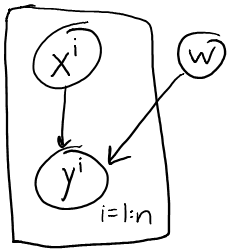
\includegraphics[scale=0.5]{contents/plate.png}\\
Training DAGs decomposes into d supervised learning problems\\
Parameter learning - fit each $\Pr(x_j\mid \text{pa}(x_j))$ independently\\
\subsection*{UGMs}
Dsb as product of non-negative potentials over subsets of variables\\
\[\Pr(x_1,x_2,\dots,x_d)\propto\prod_c \phi_c(x_c)\]
Common choice is pairwise UGM
\[\Pr(x_1,x_2,\dots,x_d)
\propto \prod_{j=1}^d \phi_j(x_j)\prod_{(i,j)\in\varepsilon} \psi_{i,j}(x_i,x_j)\]
\subsection*{Ising Model}
\[\phi_j(x_j)=\exp(w_jx_j), \phi_{ij}(x_i,x_j)=\exp(v_{ij}x_i x_j)\]
Log-linear models use $\exp$(linear) potentials\\
Often write log-linear UGMs in exp family form
\[\Pr(x\mid w)=\frac{\exp(w^T F(x))}{Z(w)}\]
\subsection*{Learning Log-Linear UGMs}
Convex NLL trained with gradient descent, 
but gradient requires inference, normalizing constant\\
\[\nabla_w-\log\Pr(x\mid w)=-F(x)+\mathbb{E}_{x\mid w}[F(x)]\]
Approx training methods include pseudolikelihood (objective fn) and variational methods\\
pseudolikelihood turns learning into $d$ single-variables problem\\
\[\Pr(x_1,\dots,x_d)\approx \prod_{j=1}^d \Pr(x_j\mid x_{\text{nei}(j)})\]
\subsection*{Younes Algorithm}
Younes algo for MCMC within SGD
\begin{enumerate}
    \item Run Gibbs sampling for a short time starting from $x_{k-1}$ with current $w^k$. e.g. 1 pass to generate $x^k$
    \item SGD Update: 
    \[w^{k+1}=w^k+\alpha_k(F(x)-F(x^k))\]
\end{enumerate}
\subsection*{Inference Tasks}
\begin{enumerate}
    \item Compute $\Pr(x)$ for an assignment to variables $x$.
    \item Generate sample $x$.
    \item Compute univariate marginals $\Pr(x_j)$.
    \item Compute decoding $\argmax_x\Pr(x)$.
    \item Compute univariate conditional $\Pr(x_j\mid x_{j'})$.
\end{enumerate}
\subsection*{Conditional Random Fields}
\[\Pr(y\mid x,w)=\frac{1}{Z(x,w)}\exp(w^T F(x,y))\]
Generalize logistic regression\\
Add features to UGM\\
\[\Pr(y_1,\dots,y_k\mid x_1,\dots,x_k)
\propto \exp(\sum_{c=1}^k y_c w^T x_c + \sum_{(c,c')\in E}y_c y_{c'}v)\]
Multi-label model explicitly models label dependencies\\
Deep structured models learn features in UGMs
\subsection*{Inference in Graphical Models}
Markov chain inference methods extend to trees for DAGs and UGMs\\
General Graphs: Inference can be hard in DAGs/UGMs\\
Uncond. sampling and learning easy in DAGs\\
Exact inference in discrete DAGs easy for trees - exponential in "treewidth" of graph
\subsection*{Need UGMs in NNs?}
Factor 1: Data Size
\begin{enumerate}
    \item Small dataset: Helpful to have direct dependencies
    \item Large dataset: Hidden layers should reflect
\end{enumerate}
Factor 2: Evaluate Model
\begin{itemize}
    \item If measure "how many pixels right", UGMs may not help.
    \item If measure "get whole sentence right", UGMs may help.
\end{itemize}